%==============================================================================
% Báo cáo Chuyên đề — An toàn Thông tin (KMA)
% "Nghiên cứu cơ chế phát hiện tấn công leo thang đặc quyền trong môi trường
%  Multi-tenant Kubernetes dựa trên phân tích System Calls"
%  (DeSFAM được dùng làm công trình tham chiếu cho thiết kế lõi phát hiện)
% Học viên: Nguyễn Ngọc Hoài — CHAT4P006
%
% Định dạng: báo cáo học thuật một cột, tiếng Việt.
% Biên dịch: XeLaTeX (qua Docker) — chạy ./build.sh
%==============================================================================
\documentclass[12pt,a4paper]{article}

% --- Lề trang ----------------------------------------------------------------
\usepackage[margin=2.5cm]{geometry}
\setlength{\parskip}{0.4em}

% --- Phông chữ Unicode (XeLaTeX): Latin Modern hỗ trợ dấu tiếng Việt ----------
\usepackage{fontspec}
\setmainfont{lmroman10}[
  Extension      = .otf,
  UprightFont    = *-regular,
  BoldFont       = *-bold,
  ItalicFont     = *-italic,
  BoldItalicFont = *-bolditalic,
]

% --- Gói cốt lõi -------------------------------------------------------------
\usepackage{graphicx}
\usepackage{amsmath,amssymb}
\usepackage{booktabs}
\usepackage{multirow}
\usepackage{array}
\usepackage{xcolor}
\usepackage[hidelinks]{hyperref}
\usepackage{url}
\usepackage{listings}
\usepackage{enumitem}

% --- Nhãn tiếng Việt ---------------------------------------------------------
\renewcommand{\abstractname}{Tóm tắt}
\renewcommand{\figurename}{Hình}
\renewcommand{\tablename}{Bảng}
\renewcommand{\refname}{Tài liệu tham khảo}
\renewcommand{\contentsname}{Mục lục}
\renewcommand{\appendixname}{Phụ lục}
\renewcommand{\listfigurename}{Danh mục hình vẽ}
\renewcommand{\listtablename}{Danh mục bảng}

% --- Kiểu trình bày mã lệnh --------------------------------------------------
\definecolor{codebg}{rgb}{0.96,0.96,0.96}
\lstset{
  basicstyle=\ttfamily\footnotesize,
  breaklines=true,
  frame=single,
  backgroundcolor=\color{codebg},
  columns=fullflexible,
  keepspaces=true,
  showstringspaces=false,
}

\begin{document}

%==============================================================================
% TRANG BÌA
%==============================================================================
\begin{titlepage}
\centering
{\large\bfseries HỌC VIỆN KỸ THUẬT MẬT MÃ}\\[2pt]
{\large\bfseries KHOA AN TOÀN THÔNG TIN}\\[6pt]
\rule{\textwidth}{0.8pt}\\[2.2cm]

{\Large\bfseries BÁO CÁO CHUYÊN ĐỀ}\\[6pt]
{\large An toàn Thông tin}\\[2.4cm]

{\large\itshape Đề tài}\\[10pt]
{\LARGE\bfseries Nghiên cứu cơ chế phát hiện tấn công leo thang\\[4pt]
đặc quyền trong môi trường Multi-tenant Kubernetes\\[4pt]
dựa trên phân tích System Calls}\\[2.6cm]

\begin{tabular}{rl}
  \textbf{Giảng viên hướng dẫn} & : TS. Nguyễn Văn Dũng\\[5pt]
  \textbf{Học viên thực hiện}   & : Nguyễn Ngọc Hoài --- CHAT4P006\\[5pt]
  \textbf{Lớp}                  & : CHAT4P\\
\end{tabular}

\vfill
{\large Hà Nội, tháng 6 năm 2026}
\end{titlepage}

%==============================================================================
% PHẦN ĐẦU: Tóm tắt, Mục lục, Danh mục
%==============================================================================
\pagenumbering{roman}

\begin{abstract}
Trong môi trường \emph{multi-tenant Kubernetes}, nhiều người thuê (tenant) bị cô
lập bằng không gian tên (namespace) nhưng vẫn \emph{chia sẻ chung một nhân} hệ điều
hành; do đó lời gọi hệ thống (syscall) trở thành bề mặt tấn công trọng yếu cho
\emph{leo thang đặc quyền} và thoát container---kẻ tấn công vượt qua ranh giới
tenant để chiếm quyền trên máy chủ. Báo cáo chuyên đề này nghiên cứu một
\emph{cơ chế phát hiện} các tấn công leo thang đặc quyền dựa trên phân tích syscall
thời gian thực. Cơ chế kế thừa thiết kế lõi phát hiện bất thường của công trình
tham chiếu DeSFAM~\cite{desfam_original} (SyscallAD: Bộ mã hóa biến phân tự động VAE
hợp nhất với Rừng cô lập iForest), trong đó các đặc trưng \emph{hiện diện của syscall
đặc quyền} (\texttt{ptrace}, \texttt{setuid/capset}, \texttt{setns},
\texttt{unshare}, \texttt{mount}, \texttt{bpf}, nạp mô-đun nhân) chính là tín hiệu
hành vi của leo thang đặc quyền. Mô hình được huấn luyện trên bộ dữ liệu công khai
DongTing~\cite{ref26_dongtingdataset} và được hiện thực hóa thành một bộ phát hiện
chạy trực tiếp: cảm biến syscall dùng Tetragon~\cite{tetragon} (eBPF) giám sát theo
namespace trên cụm Kubernetes, đẩy cảnh báo qua Prometheus/Grafana. Toàn bộ quy
trình huấn luyện và suy luận được đóng gói bằng Docker để bảo đảm khả năng tái lập.
Trên DongTing, mô hình VAE đạt AUC kiểm định $0{,}944$; tập hợp VAE\,+\,iForest đạt
AUC kiểm định $\approx 0{,}95$ và AUC trên tập kiểm tra $0{,}835$ (F1 $0{,}417$ tại
ngưỡng bảo thủ chọn trên tập kiểm định). Khi triển khai trực tiếp, điểm bất thường
tách biệt rõ giữa khối lượng công việc lành tính ($\le 0{,}19$) và các kịch bản leo
thang đặc quyền/thoát container mô phỏng theo các họ CVE thực
(\mbox{CVE-2021-4034}, \mbox{CVE-2022-0847}, \mbox{CVE-2019-5736}) trong namespace
thử nghiệm ($0{,}278$--$0{,}930$), cho phép một ngưỡng vận hành $T_0 = 0{,}25$ phát
hiện tấn công thời gian thực. Báo cáo cũng đối chiếu trung thực cơ chế đề xuất với
số liệu công bố của DeSFAM, chỉ ra các điểm tương đồng và khác biệt, cùng bài học
then chốt về căn chỉnh không gian đặc trưng giữa huấn luyện và phục vụ.

\end{abstract}

\noindent\textbf{Từ khóa:} leo thang đặc quyền, multi-tenant Kubernetes, bảo mật
container, lời gọi hệ thống, eBPF, Tetragon, phát hiện bất thường, Bộ mã hóa biến
phân tự động (VAE), Rừng cô lập, DongTing, DeSFAM.

\clearpage
\tableofcontents
\clearpage
\listoffigures
\listoftables
\clearpage

\pagenumbering{arabic}

\section{Mở đầu}
\label{sec:intro}

\subsection{Bối cảnh và động cơ}
Kubernetes đã trở thành nền tảng điều phối container phổ biến nhất cho điện toán
đám mây hiện đại. Trong mô hình triển khai \emph{multi-tenant} (nhiều người thuê),
các tenant được cô lập \emph{mức logic} bằng không gian tên (namespace), hạn ngạch
tài nguyên và chính sách mạng---nhưng tất cả vẫn \emph{chia sẻ chung một nhân} hệ
điều hành của nút (node). Khác với máy ảo, ranh giới cô lập giữa các tenant vì thế
mỏng hơn nhiều và hội tụ tại một điểm duy nhất: giao diện lời gọi hệ thống
(syscall)---ranh giới giữa không gian người dùng và nhân~\cite{ref1_jarkas_survey,
ref3_sultan_survey}.

Hệ quả là \emph{leo thang đặc quyền} (privilege escalation) và \emph{thoát
container} (container escape) trở thành lớp mối đe dọa nguy hiểm nhất trong môi
trường multi-tenant: một tenant bị xâm phạm có thể lạm dụng syscall đặc quyền để
chiếm quyền \texttt{root} trên nút và phá vỡ cô lập, ảnh hưởng tới mọi tenant khác
trên cùng nút~\cite{ref5_combe_docker}. Các họ lỗ hổng tiêu biểu---PwnKit
(\mbox{CVE-2021-4034}), Dirty~Pipe (\mbox{CVE-2022-0847}), thoát \texttt{runc}
(\mbox{CVE-2019-5736})---đều để lại \emph{dấu vết hành vi} ở tầng syscall (gọi
\texttt{ptrace}, \texttt{setuid}/\texttt{capset}, \texttt{unshare}/\texttt{setns},
\texttt{mount}, nạp mô-đun nhân, \texttt{bpf}\dots). Các cơ chế tĩnh như hồ sơ
seccomp khó duy trì, dễ chặn nhầm thao tác hợp lệ hoặc bỏ sót tấn công nhiều bước,
và không nhận thức được \emph{chuỗi} hành vi đặc trưng cho leo thang đặc quyền.

Một hướng tiếp cận thích nghi đã được công trình tham chiếu
DeSFAM~\cite{desfam_original} đề xuất: kết hợp lập hồ sơ syscall lai (tĩnh + động),
phát hiện bất thường bằng học máy độ trễ thấp (mô-đun \emph{SyscallAD} dùng VAE và
iForest), tính điểm rủi ro theo ngữ cảnh (ánh xạ MITRE ATT\&CK, tương quan CVE) và
thực thi trong nhân qua eBPF/LSM. Tuy nhiên DeSFAM đánh giá trên hạ tầng riêng,
không công bố mã nguồn đầy đủ và không đặt trọng tâm vào ngữ cảnh \emph{multi-tenant
Kubernetes}. Chuyên đề này kế thừa thiết kế lõi phát hiện của DeSFAM làm
\emph{tham chiếu} và xây dựng một cơ chế phát hiện leo thang đặc quyền vận hành
trực tiếp trong Kubernetes.

\subsection{Mục tiêu và phạm vi báo cáo}
Báo cáo chuyên đề này trình bày một \emph{cơ chế phát hiện tấn công leo thang đặc
quyền} cho môi trường multi-tenant Kubernetes dựa trên phân tích syscall, xây dựng
trên nền các nghiên cứu liên quan---trọng tâm là công trình tham chiếu
DeSFAM~\cite{desfam_original}. Đây là một báo cáo môn học theo hướng nghiên cứu
chủ đề: hệ thống hóa cơ sở lý thuyết, thiết kế và hiện thực hóa cơ chế, rồi đánh
giá thực nghiệm. Cụ thể, báo cáo:
\begin{enumerate}[label=(\roman*)]
  \item Xây dựng lõi phát hiện bất thường syscall (VAE + iForest, hợp nhất tập
        hợp) theo thiết kế tham chiếu SyscallAD của DeSFAM~\cite{desfam_original},
        trong đó các đặc trưng \emph{hiện diện của syscall đặc quyền} đóng vai trò
        tín hiệu chính cho leo thang đặc quyền; huấn luyện và kiểm chứng ngoại tuyến
        trên bộ dữ liệu công khai DongTing~\cite{ref26_dongtingdataset};
  \item Hiện thực hóa cơ chế thành một bộ phát hiện \emph{trực tiếp} trong
        Kubernetes: thu thập syscall theo namespace (tenant) bằng
        Tetragon~\cite{tetragon} (eBPF), trích đặc trưng theo cửa sổ trượt giống hệt
        lúc huấn luyện, chấm điểm và phát cảnh báo qua Prometheus/Grafana;
  \item Đánh giá khả năng phân tách lành tính/tấn công trên các kịch bản leo thang
        đặc quyền mô phỏng theo CVE thực, và đối chiếu trung thực với số liệu công
        bố của công trình tham chiếu.
\end{enumerate}

\subsection{Nội dung và bố cục báo cáo}
Báo cáo tập trung vào lớp phát hiện (không bao gồm khâu chặn nội tuyến trong nhân)
và trình bày các nội dung chính sau:
\begin{itemize}[leftmargin=1.6em]
  \item Một cơ chế phát hiện leo thang đặc quyền cho multi-tenant Kubernetes dựa
        trên phân tích syscall, với quy trình huấn luyện \emph{hoàn toàn bằng
        Docker}, có thể chạy lại từ đầu và lưu vết kết quả số (\texttt{results.json}).
  \item Một bộ phát hiện trực tiếp dựa trên Tetragon/eBPF giám sát theo namespace
        trên Kubernetes, cho thấy thiết kế tham chiếu DeSFAM khả thi trong môi
        trường vận hành thực.
  \item Một đối chiếu \emph{trung thực} giữa cơ chế đề xuất và số liệu công bố của
        DeSFAM, cùng bài học về căn chỉnh ``bảng chữ cái cảm biến'' (sensor alphabet)
        giữa huấn luyện và phục vụ.
\end{itemize}

Phần còn lại của báo cáo được tổ chức như sau: Mục~\ref{sec:related} trình bày cơ
sở lý thuyết và công trình liên quan; Mục~\ref{sec:methodology} mô tả thiết kế cơ
chế phát hiện; Mục~\ref{sec:setup} trình bày triển khai và thiết lập thực nghiệm
bằng Docker/Kubernetes; Mục~\ref{sec:evaluation} báo cáo kết quả và đánh giá (bao
gồm thảo luận và hạn chế); Mục~\ref{sec:conclusion} kết luận.

\section{Cơ sở lý thuyết và công trình liên quan}
\label{sec:related}

\subsection{Leo thang đặc quyền trong multi-tenant Kubernetes}
Trong cụm Kubernetes nhiều người thuê, các tenant được cô lập mức logic bằng
namespace nhưng chia sẻ chung nhân của nút. Bề mặt nguy hiểm nhất là \emph{leo
thang đặc quyền} và \emph{thoát container}: tận dụng lỗ hổng nhân hoặc cấu hình
sai (capabilities dư thừa, mount host-path, \texttt{ptrace}, \texttt{unshare}/
\texttt{setns}, nạp mô-đun nhân) để vượt ranh giới tenant và chiếm quyền trên
nút~\cite{ref5_combe_docker}. Mọi con đường này đều biểu hiện thành các
\emph{chuỗi syscall đặc quyền} đặc trưng, nên phân tích syscall là điểm quan sát
tự nhiên để phát hiện chúng.

\subsection{Bảo mật lời gọi hệ thống cho container}
Trong mô hình chia sẻ nhân, nhân Linux phơi bày hàng trăm syscall, phần lớn không
cần thiết cho một khối lượng công việc cụ thể, làm phình to bề mặt tấn
công~\cite{ref11_shu_security}. Các cơ chế truyền thống (seccomp, AppArmor,
SELinux) lọc theo chính sách tĩnh nên: (1) không thích nghi với hành vi thời gian
chạy; (2) thiếu nhận thức về \emph{chuỗi} syscall nên mù với tấn công nhiều bước;
và (3) tốn chi phí cấu hình thủ công ở quy mô lớn.

\subsection{Sinh danh sách syscall và lọc động}
Confine~\cite{ref31_confine} dùng phân tích tĩnh để rút gọn hồ sơ seccomp (SRR
$\approx 47{,}6\%$) nhưng không thích nghi thời gian chạy.
Prof-gen~\cite{ref36_profgen} kết hợp theo dõi lúc khởi động với đồ thị lời gọi
tĩnh, vẫn bỏ sót thay đổi hành vi về sau. Optimus~\cite{ref27_optimus} và
KubeRosy~\cite{ref29_kuberosy} dùng eBPF để cập nhật chính sách thời gian chạy,
song Optimus cần phê duyệt thủ công và KubeRosy gắn chặt với Kubernetes.
NIMOS~\cite{ref38_nimos} đánh giá giá trị của lọc dựa trên chuỗi. DeSFAM định vị
mình ở chỗ hợp nhất cả ba: lập hồ sơ lai, phát hiện bất thường học máy, và thực
thi trong nhân.

\subsection{Phát hiện xâm nhập dựa trên chuỗi syscall}
Hướng phát hiện bất thường dựa trên chuỗi syscall có lịch sử lâu dài, khởi nguồn
từ ``a sense of self''~\cite{forrest1996sense,hofmeyr1998ids} và các mô hình thay
thế~\cite{warrender1999detecting}, cùng cảnh báo kinh điển về tấn công bắt
chước~\cite{wagner2002mimicry}. Các hướng hiện đại gồm phương pháp ngữ
nghĩa~\cite{creech2014semantic}, túi lời gọi (BoSC) cho
container~\cite{abed2015bag}, và học sâu một lớp/biến phân như
DAGMM~\cite{zong2018dagmm}, Deep SVDD~\cite{ruff2018deepsvdd},
HIDS học sâu~\cite{haider2021deep}. Riêng cho container có các đánh giá phát hiện
bất thường~\cite{castanhel2021peek} và ngữ cảnh hóa syscall~\cite{elkhairi2022chids},
cũng như tập hợp Random/Isolation Forest~\cite{bsoul2022ensemble}. SyscallAD của
DeSFAM nằm trong dòng này: hợp nhất VAE~\cite{vae_kingma} (lỗi tái cấu trúc) với
iForest~\cite{iforest_liu} (ngoại lệ thống kê), bổ sung khớp mẫu lành tính bằng
PrefixSpan~\cite{prefixspan_pei}.

\subsection{Bộ dữ liệu DongTing}
DongTing~\cite{ref26_dongtingdataset} là bộ dữ liệu quy mô lớn gồm các chuỗi
syscall của nhân Linux được gán nhãn bình thường/độc hại (theo các bản vá lỗi
syzkaller), thích hợp cho huấn luyện và xác nhận bộ phát hiện bất thường. Chuyên
đề này dùng DongTing làm nguồn dữ liệu ngoại tuyến duy nhất, đúng như DeSFAM.

\subsection{eBPF và Tetragon}
eBPF cho phép nạp logic giám sát/thực thi an toàn vào nhân tại các điểm vào syscall
với chi phí thấp~\cite{ref20_bpf_security}. DeSFAM dùng eBPF/LSM để chặn nội tuyến.
Trong chuyên đề này, thay vì tự viết chương trình eBPF, chúng tôi dùng
Tetragon~\cite{tetragon} (thuộc hệ sinh thái Cilium~\cite{cilium})---một lớp quan
sát và thực thi bảo mật dựa trên eBPF cho Kubernetes---làm \emph{cảm biến syscall}
phát sự kiện qua gRPC. Đây là lựa chọn thực dụng để hiện thực hóa lớp thu thập của
DeSFAM mà không cần sửa nhân.

\subsection{Vị trí của chuyên đề}
Chuyên đề kế thừa DeSFAM như một \emph{công trình tham chiếu} cho thiết kế lõi phát
hiện bất thường syscall, và vận dụng nó để xây dựng một \emph{cơ chế phát hiện leo
thang đặc quyền} cho ngữ cảnh multi-tenant Kubernetes---một ngữ cảnh mà DeSFAM
không đặt trọng tâm. Đóng góp nằm ở chỗ: (i) định vị các đặc trưng syscall đặc
quyền làm tín hiệu cho leo thang đặc quyền; (ii) hiện thực hóa cơ chế thành một bộ
phát hiện trực tiếp giám sát theo namespace trên Tetragon/Kubernetes, lấp khoảng
trống ``từ mô phỏng đến triển khai''; và (iii) đối chiếu trung thực hiệu năng với
số liệu công bố của công trình tham chiếu.

\section{Thiết kế cơ chế phát hiện}
\label{sec:methodology}

\subsection{Tổng quan cách tiếp cận}
Cơ chế phát hiện leo thang đặc quyền được thiết kế theo nguyên tắc
\emph{huấn luyện-rồi-phục-vụ}: lõi phát hiện bất thường syscall (SyscallAD) kế thừa
thiết kế của công trình tham chiếu DeSFAM~\cite{desfam_original}, với bộ dữ liệu,
định nghĩa đặc trưng và giao thức đánh giá được cố định để có thể đối chiếu trực
tiếp với số liệu công bố. Thành phần phục vụ trực tiếp giám sát theo namespace
(tenant) trên Kubernetes nhằm kiểm chứng tính khả thi triển khai của cơ chế.

\subsection{Kiến trúc tổng thể}
Hình~\ref{fig:arch} mô tả kiến trúc ba mô-đun (giai đoạn) theo công trình tham
chiếu: (1) lập hồ sơ/danh sách truy cập syscall lai; (2) phát hiện bất thường
\emph{SyscallAD}; (3) thực thi thích ứng/phản ứng. \textbf{Trọng tâm của chuyên đề
là mô-đun SyscallAD (Giai đoạn~2)}; đây cũng là phần được hiện thực hóa và đánh giá
trọn vẹn. Hai mô-đun còn lại chỉ được \emph{điểm qua}: Giai đoạn~1 (sinh danh sách
truy cập tĩnh+động, hồ sơ seccomp, lọc theo CVE) được tóm tắt ở
Mục~\ref{sec:related} và không được hiện thực hóa lại; ở Giai đoạn~3 chuyên đề chỉ
tận dụng lớp thu thập/cảnh báo (Tetragon ghi nhật ký, phát cảnh báo), còn cơ chế
chấm điểm rủi ro (ánh xạ MITRE ATT\&CK) và chặn nội tuyến trong nhân bằng eBPF/LSM
được nêu là hướng mở rộng chứ không thuộc phạm vi nghiên cứu chính.

\begin{figure}[htbp]
  \centering
  
\includegraphics[width=\linewidth]{figures/desfam-architecture}
  \caption{Kiến trúc cơ chế phát hiện (kế thừa thiết kế tham chiếu DeSFAM): cảm
           biến syscall (eBPF/Tetragon) giám sát theo namespace $\to$ trích đặc
           trưng theo cửa sổ trượt $\to$ SyscallAD (VAE + iForest) $\to$ chấm điểm
           rủi ro và phản ứng. Mũi tên ngoại tuyến: huấn luyện trên DongTing; mũi
           tên trực tuyến: phục vụ trên multi-tenant Kubernetes.}
  \label{fig:arch}
\end{figure}

\subsection{Dữ liệu và tiền xử lý}
Nguồn dữ liệu ngoại tuyến là bản phát hành DongTing~\cite{ref26_dongtingdataset}
($18{,}9$ nghìn chuỗi được gán nhãn, các tệp \texttt{.log} kèm bảng phân chia
\texttt{Baseline.xlsx}). Chuỗi bình thường lưu dưới dạng \emph{ID syscall} phân
tách bằng dấu gạch đứng; chuỗi tấn công lưu dưới dạng \emph{tên syscall}. Chúng
tôi dùng bảng \texttt{syscall\_64.tbl} (x86-64, bỏ các dòng ABI x32) để ánh xạ
tên\,$\leftrightarrow$\,ID nhất quán. Phân chia theo bộ dữ liệu:
\texttt{DTDS-train} / \texttt{DTDS-validation} / \texttt{DTDS-test}.

\paragraph{Bảng chữ cái cảm biến (sensor alphabet).} Đây là quyết định thiết kế
\emph{then chốt} để tái lập thành công khâu triển khai trực tiếp. Chính sách truy
vết trực tiếp của Tetragon chỉ phát ra \textbf{23 syscall liên quan an ninh}
(\texttt{execve}, \texttt{clone}, \texttt{setuid/setgid/capset}, \texttt{openat},
\texttt{unlinkat}, \texttt{renameat2}, \texttt{mount}, \texttt{unshare},
\texttt{setns}, \texttt{pivot\_root}, \texttt{socket}, \texttt{connect},
\texttt{bind}, \texttt{mprotect}, \texttt{mmap}, \texttt{prctl},
\texttt{memfd\_create}, \texttt{splice}, \texttt{ptrace},
\texttt{init/finit\_module}, \texttt{bpf}---\emph{không} gồm
read/write/close/futex). Do đó khâu huấn luyện cũng lọc DongTing về đúng tập này
\emph{trước} khi cắt cửa sổ, để huấn luyện và phục vụ chia sẻ một không gian đặc
trưng. Nếu huấn luyện trên toàn bộ vũ trụ syscall, mọi cửa sổ trực tiếp sẽ suy
biến (lành tính $\approx$ tấn công).

\subsection{Trích đặc trưng theo cửa sổ trượt}
Mỗi cửa sổ trượt (độ dài $15$, bước nhảy $3$---giá trị mặc định) được biểu diễn
thành véc-tơ \textbf{43 chiều} (Hình~\ref{fig:fe}):
\[
[\, \text{freq}_8 \mid \text{disc}_{15} \mid \text{stats}_8 \mid \text{cat}_{10}
   \mid \text{prefixspan}_2 \,].
\]
\begin{itemize}[leftmargin=1.6em]
  \item \textbf{freq (8):} tần suất trong cửa sổ của các syscall phổ biến.
  \item \textbf{disc (15):} \emph{hiện diện nhị phân} của các syscall đặc quyền
        hiếm (ptrace/splice/unshare/setns/mount/bpf\dots)---đây là \emph{tín hiệu
        cốt lõi cho leo thang đặc quyền} (Hình~\ref{fig:privesc}), và bền với pha loãng:
        một \texttt{ptrace} đơn lẻ trong cửa sổ vẫn bật bit dù bị lẫn giữa nhiều
        syscall thông thường.
  \item \textbf{stats (8):} entropy, số phần tử duy nhất, độ dài, tần suất lớn
        nhất\dots
  \item \textbf{cat (10):} tần suất chuẩn hóa theo nhóm chức năng (tiến trình,
        tệp, bộ nhớ, mạng, tín hiệu, thời gian, IPC, an ninh, sự kiện I/O, khác).
  \item \textbf{prefixspan (2):} \texttt{[cờ-khớp, độ-dài-khớp/L]} từ việc đối
        sánh cửa sổ với một \emph{Cơ sở dữ liệu mẫu lành tính} khai phá bằng
        PrefixSpan~\cite{prefixspan_pei} trên cửa sổ huấn luyện bình thường.
  \item Đặc trưng thời gian (Δt) bị \emph{tắt} vì DongTing (\texttt{strace -v -f})
        không có dấu thời gian theo từng syscall (\texttt{has\_temporal=false}).
\end{itemize}
Chuẩn hóa bằng \texttt{RobustScaler} với phân vị $(1{,}99)$, \emph{chỉ} khớp trên
cửa sổ huấn luyện bình thường để tránh rò rỉ dữ liệu tấn công.

\begin{figure}[htbp]
  \centering
  
\includegraphics[width=\linewidth]{figures/feature-engineering}
  \caption{Quy trình kỹ thuật đặc trưng: từ chuỗi syscall thô $\to$ lọc theo bảng
           chữ cái cảm biến $\to$ cửa sổ trượt $(15,3)$ $\to$ véc-tơ 43 chiều.}
  \label{fig:fe}
\end{figure}

\begin{figure}[htbp]
  \centering
  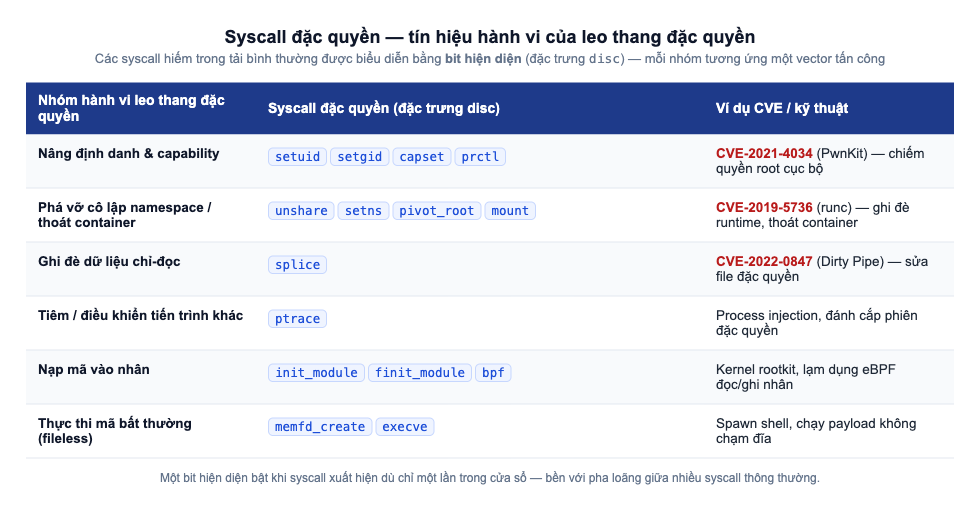
\includegraphics[width=\linewidth]{figures/privesc-syscalls}
  \caption{Ánh xạ các syscall đặc quyền (đặc trưng \texttt{disc}) sang nhóm hành vi
           leo thang đặc quyền và ví dụ CVE thực. Mỗi nhóm là một vector tấn công
           vượt ranh giới tenant; bit hiện diện của một syscall đặc quyền là tín
           hiệu phát hiện cốt lõi của cơ chế.}
  \label{fig:privesc}
\end{figure}

\subsection{Mô hình SyscallAD}
\begin{itemize}[leftmargin=1.6em]
  \item \textbf{VAE}~\cite{vae_kingma}: \texttt{hidden\_dim}=32, \texttt{latent\_dim}=8,
        huấn luyện \emph{chỉ} trên cửa sổ bình thường; điểm bất thường là lỗi tái
        cấu trúc. Huấn luyện đa hạt giống (seed 0,1,2), giữ hạt giống có AUC kiểm
        định tốt nhất để xử lý hiện tượng \emph{sụp đổ hậu nghiệm} (posterior
        collapse).
  \item \textbf{iForest}~\cite{iforest_liu}: 300 cây, \texttt{contamination}=0{,}02,
        cũng huấn luyện trên dữ liệu bình thường.
  \item \textbf{Hợp nhất tập hợp:}
        $s = 0{,}7\cdot\mathrm{RobustScale}(s_\text{VAE}) + 0{,}3\cdot\mathrm{RobustScale}(s_\text{iForest})$.
\end{itemize}

\subsection{Chọn ngưỡng (không rò rỉ)}
Ngưỡng phát hiện được chọn \emph{chỉ} trên tập kiểm định và lưu vào
\texttt{results.json}; tập kiểm tra không tham gia chọn ngưỡng. Khi phục vụ trực
tiếp, ngưỡng vận hành được hiệu chỉnh lại theo phân phối điểm quan sát trên cụm
(xem Mục~\ref{sec:evaluation}).

\subsection{Mở rộng: bộ phát hiện trực tiếp}
Thành phần suy luận đọc luồng sự kiện syscall từ Tetragon~\cite{tetragon} qua gRPC,
gom theo tiến trình, cắt cửa sổ $(15,3)$ và trích \emph{đúng} véc-tơ 43 chiều như
lúc huấn luyện (được kiểm tra ngang hàng bằng \texttt{tests/test\_feature\_parity.py}),
rồi chấm điểm bằng các mô hình đã lưu. Cảnh báo và chỉ số được phơi bày qua
Prometheus và trực quan hóa trên Grafana; nhật ký sự kiện Tetragon được thu thập
qua Loki/Promtail. Toàn bộ chạy bằng Docker/Kubernetes, không cài công cụ trực
tiếp lên máy chủ.

\section{Triển khai và thiết lập thực nghiệm}
\label{sec:setup}

\subsection{Nguyên tắc: mọi công cụ chạy bằng Docker}
Để bảo đảm khả năng tái lập và không làm ``bẩn'' máy chủ, toàn bộ chuỗi công cụ
(huấn luyện, suy luận, biên dịch báo cáo) đều chạy trong container. Quy trình
huấn luyện được đóng gói bằng \texttt{docker-compose}; bộ phát hiện trực tiếp,
Prometheus và Grafana cũng khởi chạy bằng \texttt{docker-compose}; cụm Kubernetes
thử nghiệm cài Tetragon qua script.

\subsection{Huấn luyện ngoại tuyến}
Một nguồn chân lý duy nhất là \texttt{train.py} (mọi hàm học máy, không vẽ đồ
thị); sổ tay \texttt{train\_dongting.ipynb} nhập lại từ \texttt{train.py} và bổ
sung đồ thị + bình luận học thuật. Hai chế độ luôn đồng bộ: muốn đổi thuật toán
chỉ sửa \texttt{train.py}.

\begin{lstlisting}[language=bash]
cd DeSFAM/training
# Chạy nhanh, không tương tác:
docker compose -f docker-compose.pipeline.yml run --rm train
# Hoặc tương tác (Jupyter Lab :8888):
docker compose -f docker-compose.pipeline.yml up jupyter
\end{lstlisting}

Đầu ra (lưu vào \texttt{../model/}) gồm: bộ chuẩn hóa đặc trưng, mô hình iForest,
trọng số bộ mã hóa/giải mã VAE, các bộ chuẩn hóa điểm thành phần, tham số tập hợp
($\alpha=0{,}7$), từ vựng đặc trưng (\texttt{fe\_report.json}), và
\texttt{results.json} (chỉ số + ngưỡng + siêu tham số).

\subsection{Cấu hình tái lập (ghi trong \texttt{results.json})}
Bảng~\ref{tab:config} liệt kê cấu hình thí nghiệm được lưu vết tự động, giúp người
đánh giá đối chiếu chính xác.

\begin{table}[htbp]
  \centering
  \caption{Cấu hình thí nghiệm tái lập (trích \texttt{results.json}).}
  \label{tab:config}
  \begin{tabular}{ll}
    \toprule
    \textbf{Tham số} & \textbf{Giá trị} \\
    \midrule
    Thí nghiệm & \texttt{dongting\_15\_3} \\
    Số chuỗi & 18\,874 \\
    Cửa sổ trượt (độ dài, bước) & $(15,\ 3)$ \\
    Số cửa sổ huấn luyện / kiểm định / kiểm tra & 90\,456 / 896\,581 / 687\,926 \\
    Số chiều đặc trưng & 43 \\
    VAE \texttt{latent\_dim} / \texttt{hidden\_dim} & 8 / 32 \\
    iForest \texttt{contamination} & 0{,}02 \\
    Đặc trưng thời gian & không (\texttt{has\_temporal=false}) \\
    Số mẫu lành tính (PrefixSpan) & 150 \\
    \bottomrule
  \end{tabular}
\end{table}

\subsection{Triển khai trực tiếp trên multi-tenant Kubernetes}
Cụm thử nghiệm mô phỏng môi trường nhiều người thuê bằng cách cô lập tenant theo
namespace (mỗi namespace là một tenant); cảm biến giám sát syscall \emph{theo từng
namespace} để quy kết hành vi về đúng tenant. Cảm biến syscall là
Tetragon~\cite{tetragon}, cài qua script và áp một chính sách truy vết
(\texttt{syscall-ad-tracing}) chỉ phát ra 23 syscall an ninh
(Mục~\ref{sec:methodology}). Bộ phát hiện đọc sự kiện qua gRPC NodePort.

\begin{lstlisting}[language=bash]
cd DeSFAM/Kubernetes
bash tetragon/install.sh                       # cai Tetragon + NodePort
kubectl apply -f tetragon/tracing-policy.yaml  # chinh sach 23 syscall
bash deploy.sh                                 # workload lanh tinh + tan cong
\end{lstlisting}

\begin{lstlisting}[language=bash]
cd DeSFAM/inference
# Detector + Prometheus + Grafana, dung nguong van hanh da hieu chinh:
docker compose --env-file .env.uat up -d --build
\end{lstlisting}

\subsection{Khối lượng công việc và kịch bản tấn công}
Khối lượng lành tính tiêu biểu là MongoDB (truy vấn CRUD bình thường). Kịch bản
tấn công trong không gian tên \texttt{demo} mô phỏng các chuỗi đặc quyền (thực thi
shell bất thường, \texttt{ptrace}, nạp mô-đun, thao tác \texttt{mount/unshare})
phản ánh các họ CVE thoát container và leo thang đặc quyền như
CVE-2021-4034~\cite{cve_2021_4034}, CVE-2022-0847~\cite{cve_2022_0847},
CVE-2019-5736~\cite{cve_2019_5736}. Mục tiêu là quan sát \emph{độ phân tách điểm}
giữa lành tính và tấn công khi phục vụ trực tiếp, chứ không tuyên bố chặn 14/14
CVE như công trình tham chiếu (xem Mục~\ref{sec:discussion}).

\subsection{Quan sát}
Grafana (\texttt{:3000}) hiển thị điểm bất thường theo thời gian và nhật ký sự
kiện Tetragon (qua Loki); Prometheus (\texttt{:9090}) lưu chuỗi thời gian của điểm
số và cảnh báo. Đây là kênh quan sát bằng chứng cho phần triển khai trực tiếp
(Mục~\ref{sec:evaluation}).

\section{Kết quả và đánh giá}
\label{sec:evaluation}

\subsection{Hiệu lực phát hiện ngoại tuyến trên DongTing}

\subsubsection{Hiệu năng từng mô hình và tập hợp}
Bảng~\ref{tab:offline} trình bày kết quả trên tập kiểm tra DongTing (lấy trực tiếp
từ \texttt{results.json}). VAE đạt AUC kiểm định cao và ổn định qua ba hạt giống
($0{,}9426$ / $0{,}9438$ / $0{,}9430$; chọn hạt giống~1). Trên tập kiểm tra, tập
hợp đạt AUC $0{,}835$ và Average Precision $0{,}990$.

\begin{table}[htbp]
  \centering
  \caption{Hiệu năng SyscallAD trên tập kiểm tra DongTing (cửa sổ $15/3$, 43 chiều).
           Ngưỡng chọn trên tập kiểm định.}
  \label{tab:offline}
  \begin{tabular}{lccccc}
    \toprule
    \textbf{Mô hình} & \textbf{AUC} & \textbf{AP} & \textbf{F1} & \textbf{Precision} & \textbf{Recall} \\
    \midrule
    iForest          & 0{,}851 & 0{,}991 & 0{,}474 & 0{,}999 & 0{,}311 \\
    VAE              & 0{,}734 & 0{,}985 & 0{,}421 & 0{,}999 & 0{,}267 \\
    \textbf{Tập hợp} & \textbf{0{,}835} & \textbf{0{,}990} & \textbf{0{,}417} & \textbf{0{,}999} & \textbf{0{,}264} \\
    \midrule
    VAE (AUC kiểm định, hạt giống tốt nhất) & 0{,}944 & --- & --- & --- & --- \\
    \bottomrule
  \end{tabular}
\end{table}

\subsubsection{Đối chiếu với công trình tham chiếu}
Bảng~\ref{tab:compare} đối chiếu kết quả của cơ chế đề xuất với mức công bố của
công trình tham chiếu DeSFAM~\cite{desfam_original}. Có \emph{tương đồng} ở hai
điểm: (i) AUC kiểm định của VAE thậm chí cao hơn mức công bố cho thành phần VAE;
(ii) độ chính xác (precision) rất cao ($\approx 0{,}999$), khớp định hướng ``ít báo
động giả''. Tuy nhiên \emph{còn khác biệt} ở F1/Recall so với mức công bố: F1 tập
hợp của chúng tôi
$0{,}417$ so với $0{,}92$ trong công trình tham chiếu, do recall thấp ($0{,}264$) tại ngưỡng bảo
thủ chọn trên tập kiểm định (ngưỡng ưu tiên precision). Nói cách khác, mô hình
\emph{xếp hạng} bất thường tốt (AUC/AP cao) nhưng \emph{điểm chốt nhị phân} tại
một ngưỡng cố định lại bỏ sót nhiều cửa sổ tấn công.

\begin{table}[htbp]
  \centering
  \caption{Cơ chế đề xuất so với số liệu công bố của công trình tham chiếu DeSFAM
           (lõi phát hiện bất thường).}
  \label{tab:compare}
  \begin{tabular}{lcc>{\raggedright\arraybackslash}p{4.2cm}}
    \toprule
    \textbf{Chỉ số} & \textbf{DeSFAM (công bố)} & \textbf{Cơ chế đề xuất} & \textbf{Nhận định} \\
    \midrule
    AUC (tập hợp)        & 0{,}94 & 0{,}835 & Thấp hơn nhưng cùng bậc \\
    AP                   & 0{,}87 & 0{,}990 & Cao hơn (dữ liệu mất cân bằng) \\
    F1 (tấn công)        & 0{,}92 & 0{,}417 & \textbf{Còn khác biệt}---do ngưỡng ưu tiên precision \\
    VAE (AUC kiểm định)  & 0{,}747\,$^{*}$ & 0{,}944 & Cao hơn mức công bố cho VAE \\
    Precision            & cao    & 0{,}999 & Tái lập định hướng ít báo động giả \\
    \bottomrule
    \multicolumn{4}{l}{\footnotesize $^{*}$Giá trị thành phần VAE theo Bảng~1 của công trình tham chiếu; tập hợp công bố $\approx 0{,}94$.}
  \end{tabular}
\end{table}

\subsection{Triển khai trực tiếp trên multi-tenant Kubernetes}
Khi phục vụ trực tiếp, mô hình huấn luyện ngoại tuyến giữ được \emph{khả năng phân
tách} giữa lành tính và tấn công---kết quả quan trọng nhất của chuyên đề:
\begin{itemize}[leftmargin=1.6em]
  \item Khối lượng lành tính (MongoDB) có điểm bất thường $\le 0{,}19$.
  \item Các kịch bản tấn công trong không gian tên \texttt{demo} có điểm
        $0{,}278$--$0{,}930$.
\end{itemize}
Khoảng trống giữa hai phân phối cho phép đặt một \textbf{ngưỡng vận hành
$T_0 = 0{,}25$} (lưu trong \texttt{inference/.env.uat}) tách sạch hai lớp trong
môi trường thử nghiệm (Hình~\ref{fig:separation}). Đây là bằng chứng cho thấy
thiết kế DeSFAM khả thi ngoài mô phỏng: cùng một không gian đặc trưng 43 chiều,
sinh ngoại tuyến từ DongTing và trực tuyến từ Tetragon, tạo ra điểm số tương thích.

\begin{figure}[htbp]
  \centering
  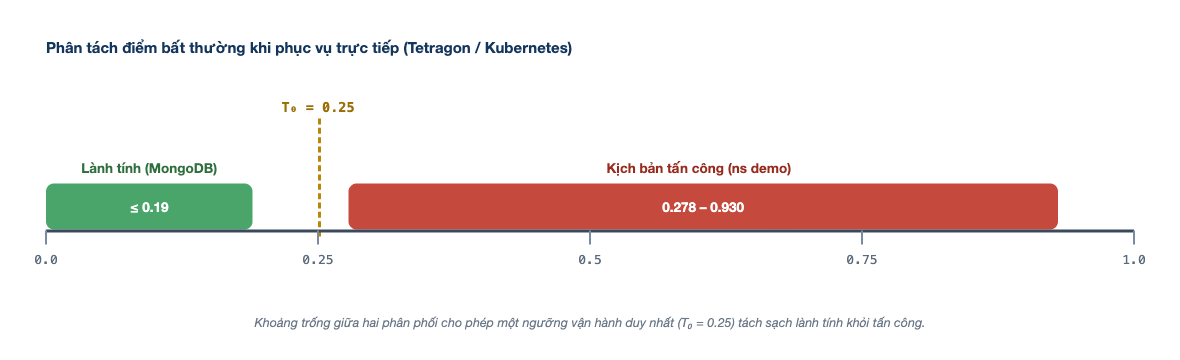
\includegraphics[width=\linewidth]{figures/live-separation}
  \caption{Phân tách điểm bất thường khi phục vụ trực tiếp qua Tetragon trên
           Kubernetes. Khối lượng lành tính (MongoDB) nằm dưới ngưỡng vận hành
           $T_0=0{,}25$, các kịch bản tấn công nằm trên---khoảng trống đủ rộng để
           một ngưỡng duy nhất tách sạch hai lớp.}
  \label{fig:separation}
\end{figure}

\begin{table}[htbp]
  \centering
  \caption{Phân tách điểm bất thường khi phục vụ trực tiếp (Tetragon/K8s).}
  \label{tab:live}
  \begin{tabular}{lcc}
    \toprule
    \textbf{Nguồn} & \textbf{Khoảng điểm} & \textbf{So với $T_0=0{,}25$} \\
    \midrule
    MongoDB (lành tính)        & $\le 0{,}19$        & Dưới ngưỡng (không báo động) \\
    Kịch bản tấn công (\texttt{demo}) & $0{,}278$--$0{,}930$ & Trên ngưỡng (báo động) \\
    \bottomrule
  \end{tabular}
\end{table}

\subsection{Điều kiện thành công của cơ chế}
Yếu tố quyết định là \textbf{căn chỉnh bảng chữ cái cảm biến} giữa huấn luyện và
phục vụ. Khi huấn luyện trên toàn bộ vũ trụ syscall (gồm read/write/close/futex
mật độ cao) trong khi Tetragon chỉ phát 23 syscall an ninh, mọi cửa sổ trực tiếp
trở nên thưa và \emph{suy biến}: điểm lành tính $\approx$ điểm tấn công, không thể
đặt ngưỡng. Sau khi buộc \texttt{train.py} lọc DongTing về đúng 23 syscall trước
khi cắt cửa sổ (\texttt{SENSOR\_ALPHABET=1}), AUC kiểm định của VAE tăng lên
$0{,}944$ (giải quyết sụp đổ hậu nghiệm) và đạt được độ phân tách trực tiếp ở
Bảng~\ref{tab:live}. Bài học: trong các hệ phát hiện bất thường \emph{huấn
luyện-rồi-phục-vụ}, sự đồng nhất không gian đặc trưng quan trọng ngang---thậm chí
hơn---kiến trúc mô hình. Tính đồng nhất này được ràng buộc bằng kiểm thử ngang
hàng \texttt{test\_feature\_parity.py} (đạt) để \texttt{train.py} và bộ trích đặc
trưng khi phục vụ sinh véc-tơ \emph{trùng khít từng bit}.

\subsection{Thảo luận và đánh giá}
\label{sec:discussion}

\subsubsection{Cơ chế đạt được gì so với công trình tham chiếu}
Cơ chế đề xuất tái hiện được \emph{định hướng và tính khả thi} của lõi phát hiện
tham chiếu DeSFAM: bộ phát hiện VAE\,+\,iForest xếp hạng bất thường tốt (AUC kiểm
định VAE $0{,}944$; AP tập hợp $0{,}990$) và giữ khả năng phân tách khi phục vụ
trực tiếp qua Tetragon. Điều \emph{chưa} đạt là các con số tuyệt đối ở chế độ phân
loại nhị phân---đặc biệt F1 $0{,}92$ và recall cao của công trình tham chiếu. Nguyên nhân khả dĩ:
(i) công trình tham chiếu
chọn ngưỡng tối ưu F1 hoặc đánh giá trên một phân chia tấn công/khối lượng khác;
(ii) khác biệt về phiên bản DongTing, cách cắt cửa sổ và tập syscall đầu vào;
(iii) công trình tham chiếu bổ sung Giai đoạn~3 (thực thi trong nhân) để đạt ``chặn 14/14 CVE''
---một chỉ số \emph{thực thi}, không phải chỉ số phân loại của riêng SyscallAD.

\subsubsection{Ý nghĩa của khoảng cách ngưỡng}
Việc AUC/AP cao nhưng F1 thấp tại ngưỡng cố định cho thấy giá trị của \emph{hiệu
chỉnh ngưỡng theo môi trường}. Ngưỡng bảo thủ chọn trên tập kiểm định ($0{,}81$
cho điểm tập hợp đã chuẩn hóa) tối đa hóa precision nên bỏ sót cửa sổ tấn công
``nhẹ''. Ngược lại, khi phục vụ trực tiếp, ngưỡng vận hành $T_0=0{,}25$ được hiệu
chỉnh theo phân phối quan sát giúp tách sạch hai lớp. Đây là một phát hiện thực
dụng: với phát hiện bất thường, hiệu chỉnh ngưỡng tại chỗ quan trọng ngang với
chất lượng mô hình.

\subsubsection{Lựa chọn thiết kế khác với công trình tham chiếu}
Chúng tôi dùng Tetragon~\cite{tetragon} làm cảm biến eBPF thay vì tự viết chương
trình eBPF/LSM. Điều này đẩy nhanh hiện thực hóa và bám hệ sinh thái Kubernetes
thực tế, nhưng cũng \emph{thu hẹp} bảng chữ cái syscall về 23 lời gọi an ninh---một
ràng buộc kéo theo phải lọc dữ liệu huấn luyện tương ứng
(Mục~\ref{sec:evaluation}). Việc thực thi/chặn trong nhân (Giai đoạn~3 đầy đủ của
DeSFAM) chưa được hiện
thực hóa; chuyên đề dừng ở phát hiện và cảnh báo.

\subsubsection{Hạn chế và đe dọa tính hợp lệ}
\begin{itemize}[leftmargin=1.6em]
  \item \textbf{Hợp lệ nội tại:} kịch bản tấn công trực tiếp là \emph{mô phỏng}
        chuỗi syscall đặc quyền, không phải khai thác CVE thực; do đó độ phân tách
        ở Bảng~\ref{tab:live} là dấu hiệu khả quan chứ chưa phải bằng chứng chặn
        khai thác thật.
  \item \textbf{Hợp lệ ngoại tại:} một khối lượng lành tính (MongoDB) và một không
        gian tên thử nghiệm chưa đại diện cho đa dạng khối lượng sản xuất; cần mở
        rộng (Nginx, Redis, Node.js\dots) như công trình tham chiếu.
  \item \textbf{Hợp lệ kết luận:} mất cân bằng lớp lớn (tỉ lệ tấn công cao trong
        tập kiểm tra cửa sổ) khiến AP cao dễ gây hiểu nhầm; chúng tôi báo cáo kèm
        AUC, precision, recall để tránh kết luận một chiều.
  \item \textbf{Hợp lệ cấu trúc:} đặc trưng thời gian bị tắt do DongTing không có
        dấu thời gian theo syscall; mô hình có thể thiếu một tín hiệu mà công trình
        tham chiếu tận dụng.
\end{itemize}

\subsubsection{Hướng cải thiện}
(1) Chọn ngưỡng tối ưu F1 và báo cáo đường cong precision--recall đầy đủ;
(2) hiện thực hóa Giai đoạn~3 (chặn bằng eBPF/LSM hoặc Tetragon Enforcement) để đo
``tỉ lệ chặn'' so sánh trực tiếp với công trình tham chiếu; (3) mở rộng tập khối lượng và dùng
khai thác CVE thực trong môi trường cách ly; (4) bổ sung đặc trưng thời gian khi
dùng cảm biến có dấu thời gian (Tetragon cung cấp), điều DongTing thiếu.

\section{Kết luận}
\label{sec:conclusion}

Chuyên đề đã nghiên cứu và hiện thực hóa một \emph{cơ chế phát hiện tấn công leo
thang đặc quyền} cho môi trường multi-tenant Kubernetes dựa trên phân tích lời gọi
hệ thống. Cơ chế kế thừa thiết kế lõi phát hiện bất thường SyscallAD (VAE + Rừng cô
lập) của công trình tham chiếu DeSFAM~\cite{desfam_original}, định vị các đặc trưng
syscall đặc quyền làm tín hiệu cho leo thang đặc quyền; huấn luyện trên bộ dữ liệu
công khai DongTing và được triển khai thành một bộ phát hiện chạy trực tiếp bằng
Tetragon/eBPF giám sát theo namespace trên Kubernetes, toàn bộ đóng gói bằng Docker
để bảo đảm tái lập.

Các kết quả chính như sau. \emph{Về phát hiện ngoại tuyến}, lõi phát hiện đạt định
hướng và khả năng xếp hạng tốt (VAE AUC kiểm định $0{,}944$, AP tập hợp $0{,}990$,
precision $0{,}999$) nhưng còn khác biệt về F1/recall so với mức công bố do ngưỡng
ưu tiên precision. \emph{Về triển khai trực tiếp}, mô hình giữ được khả năng phân
tách khi phục vụ trực tiếp (lành tính $\le 0{,}19$ so với các kịch bản leo thang
đặc quyền $0{,}278$--$0{,}930$), cho phép ngưỡng vận hành $T_0=0{,}25$. \emph{Về
điều kiện thành công}, yếu tố then chốt là căn chỉnh không gian đặc trưng (bảng chữ
cái cảm biến 23 syscall) giữa huấn luyện và phục vụ, được ràng buộc bằng kiểm thử
ngang hàng.

Tóm lại, báo cáo trình bày một cơ chế phát hiện khả thi cho leo thang đặc quyền
trong multi-tenant Kubernetes, kèm một đối chiếu \emph{trung thực} với công trình
tham chiếu: chỉ rõ điều gì tương đồng, điều gì khác biệt và vì sao, đồng thời
lấp khoảng cách ``mô phỏng $\to$ triển khai'' bằng một bộ phát hiện trực tiếp. Hướng
tiếp theo gồm chọn ngưỡng tối ưu F1, hiện thực hóa khâu chặn trong nhân (Giai đoạn~3)
để \emph{ngăn chặn} chứ không chỉ phát hiện, mở rộng khối lượng công việc đa tenant
và dùng khai thác CVE thực trong môi trường cách ly.


\bibliographystyle{IEEEtran}
\bibliography{references}

\appendix
\section{Phụ lục Tái lập Kết quả}
\label{app:repro}

Phụ lục này cho phép một người đánh giá độc lập tái lập kết quả. \emph{Mọi công cụ
chạy bằng Docker}---không cần cài đặt trực tiếp lên máy chủ (ngoài Docker và, cho
phần trực tiếp, một cụm Kubernetes có quyền nạp eBPF).

\subsection{Môi trường}
\begin{lstlisting}[language=bash]
# Yeu cau: Docker; (phan truc tiep) mot cum Kubernetes + Tetragon.
git clone <REPO_URL> && cd kma-chuyen-de
# Du lieu DongTing: nap tu cac zip trong DongTing/DB (xem README).
\end{lstlisting}

\subsection{Huấn luyện ngoại tuyến (tái lập Bảng~\ref{tab:offline})}
\begin{lstlisting}[language=bash]
cd DeSFAM/training
docker compose -f docker-compose.pipeline.yml run --rm train
# Ket qua so + nguong duoc ghi vao ../model/results.json
\end{lstlisting}

\subsection{Triển khai trực tiếp (tái lập Bảng~\ref{tab:live})}
\begin{lstlisting}[language=bash]
cd DeSFAM/Kubernetes
bash tetragon/install.sh
kubectl apply -f tetragon/tracing-policy.yaml   # 23 syscall an ninh
bash deploy.sh                                   # workload lanh tinh + tan cong

cd ../inference
docker compose --env-file .env.uat up -d --build # detector + Prometheus + Grafana
# Grafana: http://localhost:3000  (admin/admin)
\end{lstlisting}

\subsection{Kiểm tra tính nhất quán đặc trưng}
\begin{lstlisting}[language=bash]
cd DeSFAM
# Bao dam train.py va bo trich dac trung khi phuc vu sinh vec-to trung khit:
docker compose -f training/docker-compose.pipeline.yml run --rm \
  train python -m pytest tests/test_feature_parity.py -q
\end{lstlisting}

\subsection{Biên dịch báo cáo này (Docker)}
\begin{lstlisting}[language=bash]
cd Report
./build.sh        # chay XeLaTeX qua Docker texlive -> main.pdf
\end{lstlisting}


\end{document}
